\documentclass[12pt,a4paper]{article}
\usepackage[UTF8]{ctex}     %先引入ctex
\usepackage[utf8]{inputenc} %再引入inputenc
\usepackage{graphicx}
% \usepackage{lazylatex}
% \tcbuselibrary{documentation}
\usepackage{multicol}
\usepackage{tikz}
\usetikzlibrary{matrix}
\usepackage{pgfplots}
\usepackage{pgfplotstable}
\usepgfplotslibrary{colorbrewer}
\pgfplotsset{compat=1.17}
\usepackage{xcolor}
\usepackage{listings}
\usepackage{amsmath}
\usepackage{bookmark}
\usepackage{enumerate}
\usepackage{geometry}
\graphicspath{{img/}}
% 边距
\geometry{left=2.0cm,right=2.0cm,top=2.0cm,bottom=3.0cm}
% 大题
\newenvironment{problems}{\begin{list}{}{\renewcommand{\makelabel}[1]{\textbf{##1}.\hfil}}}{\end{list}}
% 小题
\newenvironment{steps}{\begin{list}{}{\renewcommand{\makelabel}[1]{(##1)\hfil}}}{\end{list}}
% 答
\providecommand{\ans}{\textbf{答}:~}
% 解
\providecommand{\sol}{\textbf{解}.~}

% \setminted{breaklines,autogobble,frame=lines,framesep=2mm,fontsize=\scriptsize}

% listings
\definecolor{grey}{rgb}{0.8,0.8,0.8}
\definecolor{darkgreen}{rgb}{0,0.3,0}
\definecolor{darkblue}{rgb}{0,0,0.3}
\lstset{%
    numbers=left, %行号
    numberstyle=\tiny\color{grey},
    showstringspaces=false,
    showspaces=false,%
    tabsize=4,%
    frame=shadowbox,%
    basicstyle={\ttfamily\scriptsize},%
    keywordstyle=\color{blue!80!black}\bfseries,%
    commentstyle=\color{green!50!blue}\itshape,%
    stringstyle=\color{green!50!black},%
    rulesepcolor=\color{gray!20!white},
    breaklines,
    columns=flexible,
    extendedchars=false,
    %mathescape=true,
    language=c,
}

\setlength{\columnsep}{3em}

\hypersetup{
	colorlinks, linkcolor=blue
}

\begin{document}
\title{\normalsize \underline{计算机系统结构(A)}\\\LARGE 实验 6}
\author{Log Creative }
\date{\today}
\maketitle

\begin{problems}
    \item[一] \textbf{向量加法}
    
	\begin{enumerate}
		\item 运行结果如下:
		
		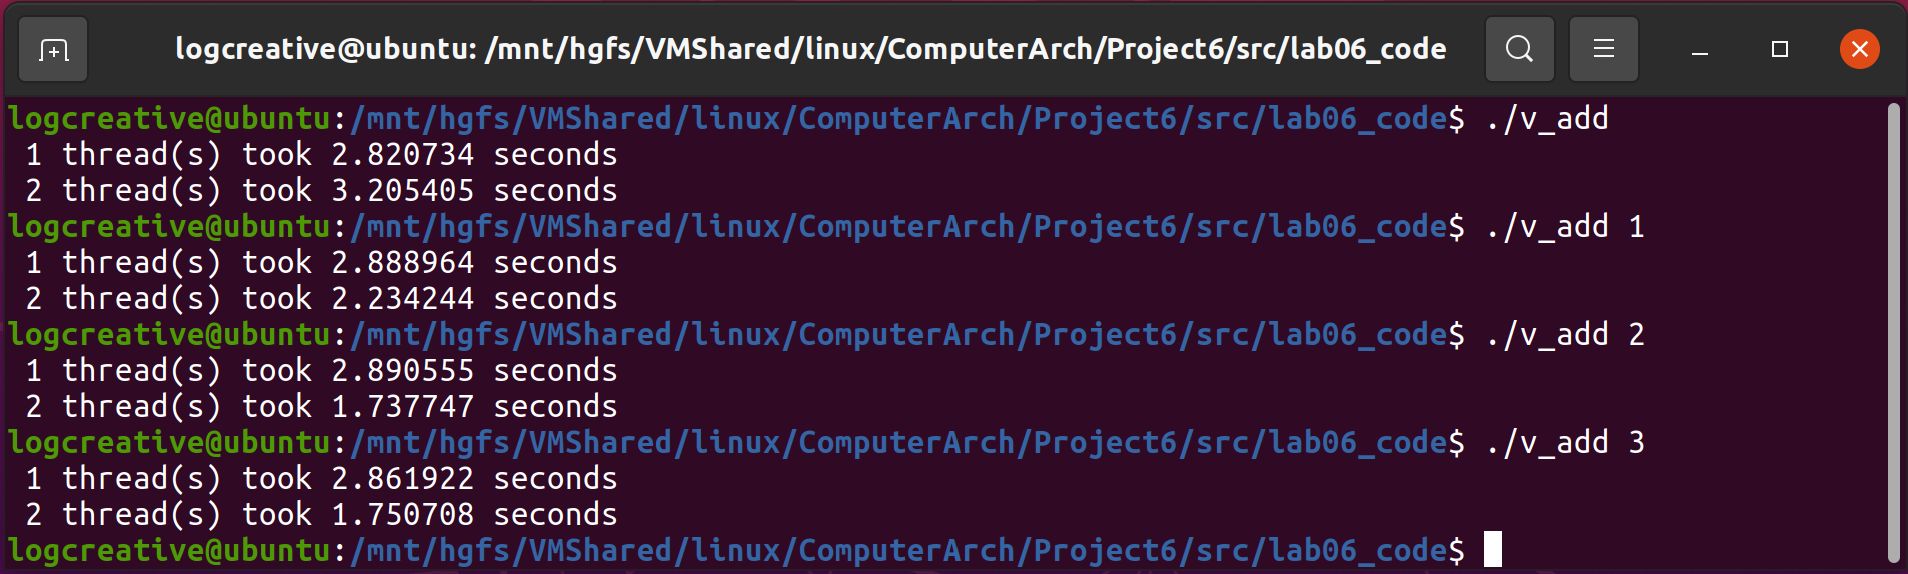
\includegraphics[width=0.9\textwidth]{add.png}

		假共享问题,访问同一个数组,导致一个处理器修改数组后,多个处理器的数组已经不再有效,需要通过广播更改数组。\verb"method_1()" 受到 cache 大小和处理器个数的影响,虽然使用了 \texttt{gap} 在一定程度上缓解了逐步访问相邻块导致的假共享,但是由于处理器仍然访问相邻块,cache大小足够小时才会有更好的性能,否则依然会 dirty。

		\begin{figure}[h]
		\begin{tikzpicture}
			\begin{axis}[ylabel={Running Time(s)},
			xlabel={method},
			symbolic x coords={method0,method1,method2,method3},
			xtick=data,ybar,width=0.45\textwidth,]
			 \pgfplotstableread {img/add.dat}{\addres};
			 \addplot+ [] table[x=method,y=thread1,] {\addres};
			 \addplot+ [] table[x=method,y=thread2,] {\addres};
			 \legend{thread 1,thread 2,}
			\end{axis}
		\end{tikzpicture}			
		\begin{tikzpicture}
			\begin{axis}[ylabel={Perf. ratio},
				xlabel={method},symbolic x coords={method0,method1,method2,method3},
			xtick=data,width=0.45\textwidth]
			 \pgfplotstableread {img/add.dat}{\addres};
			 \addplot+ [ybar,no markers] table[x=method,y=thread1,] {\addres};
			 \addplot+ [ybar,no markers] table[x=method,y=thread2,] {\addres};
			 \addplot+ [] table[x=method,y expr=\thisrow{thread1}/\thisrow{thread2}] {\addres};
			 \legend{,,Perf. ratio,}
			\end{axis}
		\end{tikzpicture}
		\caption{不同方法的性能}
		\end{figure}			

		\item 达到了同等的性能。
		\begin{lstlisting}
void method_3(double* x, double* y, double* z) {
#pragma omp parallel
{
  // your code here:
  int block = omp_get_num_threads();
  int n = omp_get_thread_num();
  int block_size = ARRAY_SIZE / block + 1;
  int low = n * block_size;
  int high = (n + 1) * block_size;
  for(int i = low; i < high && i < ARRAY_SIZE; ++i){
    z[i] = x[i] + y[i];
  }
}

}
		\end{lstlisting}
	\end{enumerate}
	
	\item[二] \textbf{点积}
	
	\begin{enumerate}
		% \item 为了更好的利用多核,在 Windows 平台上的运行结果如下:
		
		% 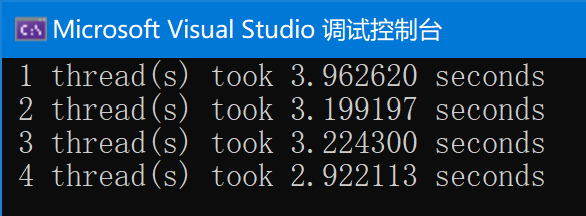
\includegraphics[width=0.4\textwidth]{dotp1.png}
		% \begin{tikzpicture}
		% 	\begin{axis}[ymin={0},
		% 	xlabel={Thread Number},
		% 	ylabel={Running Time(s)},
		% 	symbolic x coords={thread1,thread2,thread3,thread4}, xtick=data,
		% 	ybar,]
		% 	 \addplot+ [] table[x=thread,y=running,] {img/dotp.dat};
		% 	\end{axis}
		% \end{tikzpicture}

		% 在线程大于等于 2 的时候,运行时间几乎一致。
		% \item 性能没有改善,甚至会相对变差,因为增加了调用和存储局部变量的开销。

		\item 运行结果如下:
		
		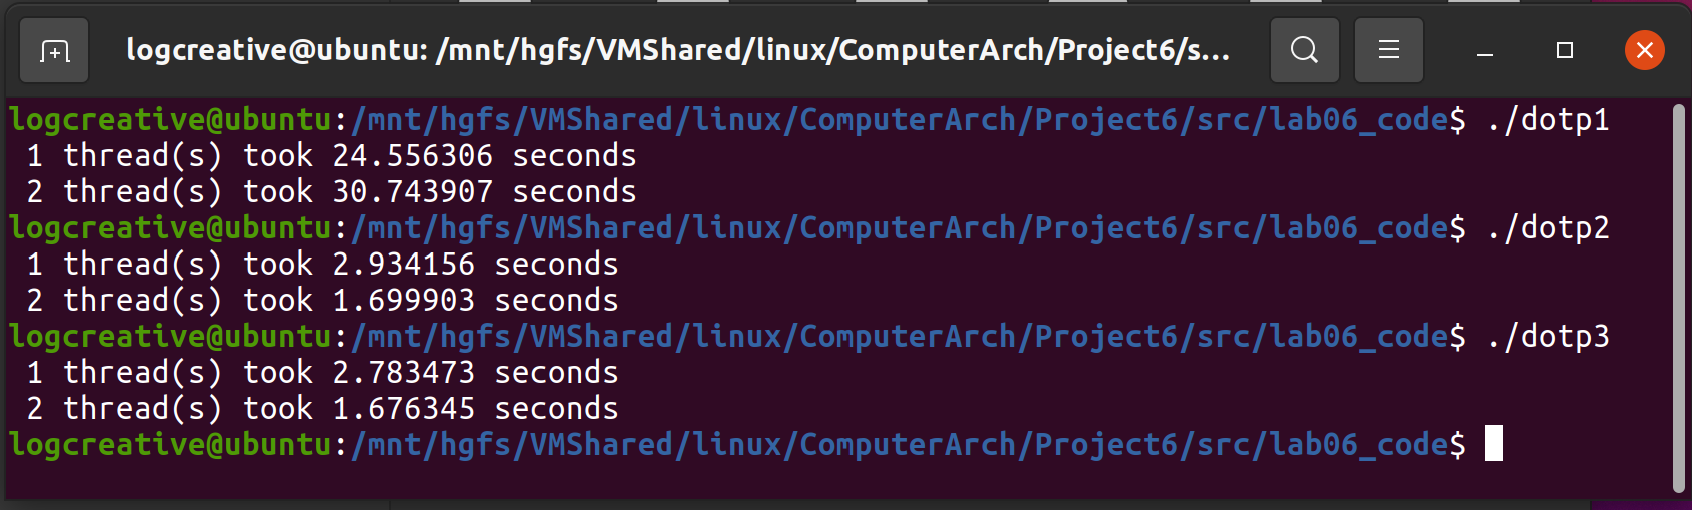
\includegraphics[width=0.8\textwidth]{dotp.png}
		
		线程数目越多,反而性能越差。当线程数增多时,进入临界区的请求就会变多,有时候反而就会因为排队时间的增长而导致较长的运行时间。

		\begin{figure}[h]
			\centering
			\begin{tikzpicture}
				\begin{axis}[ymin={0},
				xlabel={Method},
				ylabel={Running Time (s)},
				symbolic x coords={dotp1,dotp2,dotp3}, xtick=data,
				ybar,]
				 \pgfplotstableread {img/dotpl.dat}{\dotp};
				 \addplot+ [] table[x=method,y=thread1,] {\dotp};
				 \addplot+ [] table[x=method,y=thread2,] {\dotp};
				 \legend{1 thread,2 threads,}
				\end{axis}
			\end{tikzpicture}
			\caption{点积程序运行结果}
		\end{figure}

		\item 性能得到了巨大的改变。
		\begin{lstlisting}
double dotp_2(double* x, double* y) {
    double global_sum = 0.0;
    #pragma omp parallel
    {
      // your code here: modify dotp_1 to improve performance
        double local_sum = 0.0;
        #pragma omp for
        for (int i = 0; i < ARRAY_SIZE; i++) {
           local_sum += x[i] * y[i];
        }
        #pragma omp critical
            global_sum += local_sum;
    }
    return global_sum;
}
		\end{lstlisting}

		\item reduction 的作用\footnote{\href{https://hpc.llnl.gov/openmp-tutorial\#REDUCTION}{https://hpc.llnl.gov/openmp-tutorial\#REDUCTION}}:
		\begin{quotation}\itshape
			A private copy for each list variable is created and initialized for each thread. At the end of the reduction, the reduction variable is applied to all private copies of the shared variable, and the final result is written to the global shared variable.
		\end{quotation}

		和 \verb"dotp_2" 的方法几乎一致,性能与 \verb"dotp_2" 也几乎一致。

	\end{enumerate}
\end{problems}
\end{document}
